\chapter {Бекаа-82, часть 3. Величайшая битва после Кореи}
\begin{remark}
"… менее чем через минуту израильтяне поставили помехи по каналу связи с землей, и ловушка захлопнулась. МиГи остались один на один с “Орлами”.
Израильтяне наперегонки выпустили две AIM-7F - но первая в истории ракетная атака F-15 за пределами видимости провалилась, и обе “Спэрроу” потеряли цель. Сирийцы, быстро сообразив, что к чему, на форсаже стали уходить назад, в сторону границы. Оба израильских звена бросилась за ними. Сирийцы поняли, что не успеют уйти - и начался бой.

Первый F-15 довернул на пару “Миг-21” и выпустил ракету - теперь с тепловым наведением. Вскоре на месте одного из МиГов сверкнула яркая вспышка, а израильский лётчик стал первым результативным пилотом F-15 в мире. Но стоило на мгновение расслабиться, как ему в хвост начал заходить второй МиГ - только для того, чтобы быть сбитым ведомым второй пары. На этот раз “Спэрроу” не подвела. Тем временем, смешанное звено F-15 и “Кфиров” добралось до места сражения и набросилось на сирийцев. У израильтян проснулись старые инстинкты пилотов “Миражей”. Радар? Ракеты? К черту! Пушки и маневренный ближний бой!

Они спешили - слыша, что первое звено уже вступило в схватку и опасаясь, что всех сирийцев собьют до их появления. Так что лидер второй пары первого звена был очень удивлен, едва захватив в прицел МиГ, когда тот к его огромному удивлению взорвался в воздухе - его напарник, будущий первый ас F-15 оказался быстрее. Впрочем, он тут же овладел ситуацией и достал второй МиГ очередью из “Гатлинга”. Тем временем пара “Кфиров”, вступившая в бой последней, сбила еще одного - последнего в тот день ..."	
\end{remark}

Итак, 9 июня всего за час “Феда” пала. Сирийцы отправились зализывать раны - и думать, что в сложившейся ситуации делать. Надежды на новый “зонтик ПВО” не было - очевидно, что израильтяне размолотят любое сирийское ПВО вне зависимости от его состава. Правда, "отложенные" в начале войны 5 дивизионов “Квадратов” в Бекаа все-же ввели, но “Фантомы” добили их утром следующего дня, ровно тем же способом, что и предыдущие. Спровоцировали облучить радаром демонстративную группу - подавили помехами - выбили станции управления управляемым бомбами и добили пусковые. После этого сирийцы вывели уцелевшие комплексы из Ливана и больше не рисковали ими.

Приблизительно через час после первого удара по сирийской ПВО 9 июня, лавина из сотни “Фантомов” и “Кфиров” под прикрытием F-15 и F-16 вернулась в Бекаа, и приступила к нанесению ударов по сирийским войскам. “Скайхоки” были задействованы достаточно эпизодически - как правило в роли самолета непосредственной поддержки наземных войск они действовали существенно западнее, главным образом - против целей ООП. Тем более, что целям в городской застройке они могли работать существенно лучше, чем любой другой самолет.

Было понятно, что главные события происходят не в воздухе, а на земле. И, собственно, ключевая цель авиации - максимально упростить задачу своим наземным войскам и усложнить - чужим. Сирийское командование на земле действовало грамотно - понимая, что остановить наступление израильтян нереально, они постарались максимально его замедлить - до тех пор, пока под давлением ООН не будет подписано мирное соглашение. Всем было понятно, что прекращение огня - вопрос считанных дней. И обе стороны стремились по максимуму их использовать.

\begin{figure}[h!tb] 
	\centering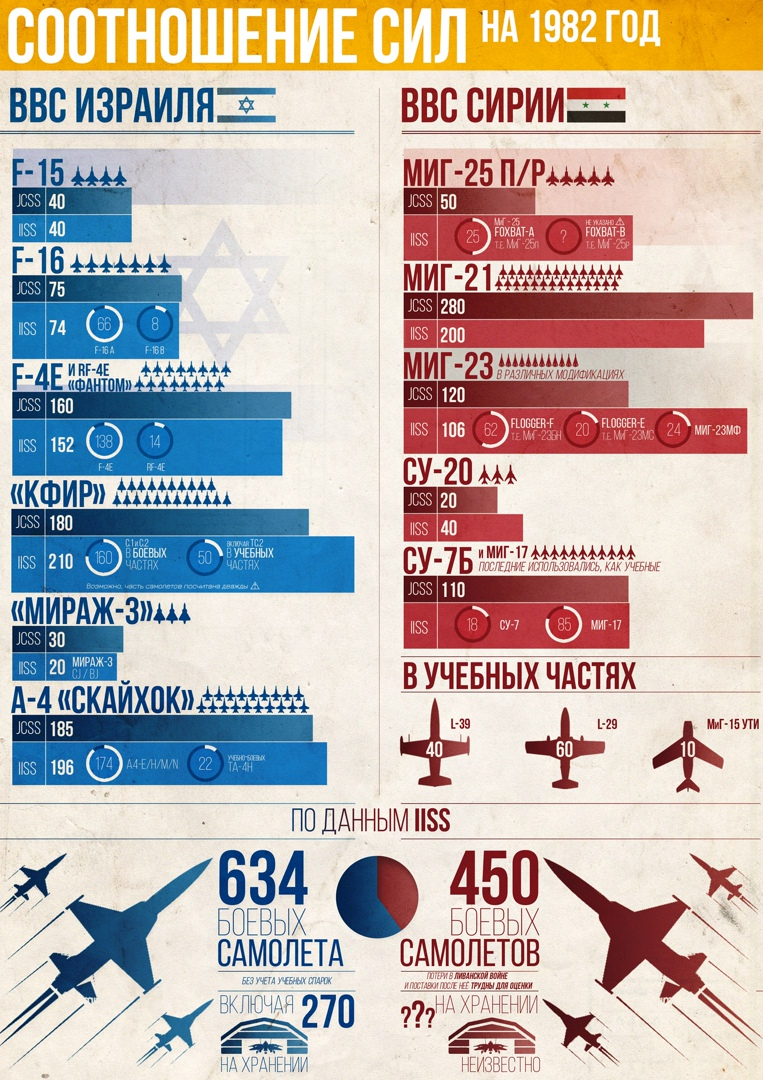
\includegraphics[scale=0.5]{Bekaa_3/BRm_1jpZcUs.jpg}
	%	\label{fig:scipion} % Unique label used for referencing the figure in-text\end{document}
	%	%\addcontentsline{toc}{figure}{Figure \ref{fig:placeholder}} % Uncomment to add the figure to the table of contents%----------------------------------------------------------------------------------------
	\caption{РЛС П-15, рабочая лошадка сирийских РТВ}%	CHAPTER 2
\end{figure}

Итак, основой сирийской наземной тактики были засады и минирование. Израильтяне же в это время занимались в основном тем, что стояли в пробках. А ввиду редкостной паршивости тамошних дорог и большого объема техники, отправленной в Ливан, дороги там стояли хуже, чем Проспект Мира утром. А стоящая техника - это что? Это идеальная мишень! Соответственно и была поставлена задача сирийцам - атаковать движущиеся на марше колонны (на самом деле стоящие в глухих пробках колонны), места сосредоточения техники, места отдыха, части технического обеспечения и так далее.

Тут у сирийцев встал вопрос, где брать целеуказание? Разведка работала ужасно, сирийские самолеты над Ливаном летали нечасто и тяжело - приходилось ориентироваться на микст агентурной разведки (!) и информации от сирийских же частей в Ливане. С авианаводчиками тоже не сложилось - если у израильтян огромное количество пехотных офицеров прошло соответствующий курс, то у сирийцев грамотных в этом людей практически не было. В итоге, проблему наведения на цель сирийцы так и не решили. В отличие от них, у израильтян такой проблемы не было - время пребывания над целью для них ограничивалось лишь запасом топлива и скоростью прибытия следующего звена. То есть у них всегда была возможность сделать лишний круг над целью, точно ее идентифицировать, получить информацию с земли и неторопясь отбомбиться. Ну, если хватало топлива.

Зато специализированных бомбовозов у сирийцев было множество - старший брат поставил им несколько эскадрилий МиГ-23БН и СУ-22 (экспортных СУ-17). По своим ударным возможностям, эти самолеты были достаточно близки к “Фантомам” - правда летчики Фантомов при необходимости могли за себя постоять гораздо лучше, сказывалась совершенно иная подготовка пилотов. Сирийские пилоты бомбардировочных эскадрилий практически не учились вести воздушный бой, так что разница сказалась быстро.

Итак, наступило 10 июня. Война с Израилем стала реальностью, а ее первый день - катастрофой. Пути к отступлению не было.

Для сирийцев стало очевидным, что их тактика предыдущего дня не работает - МиГ-23 не смогли навязать бой новым израильским самолетам, и понесли тяжелые потери. Становилось понятно, что если они продолжат терять самолеты с той же скоростью, 17-я авиабригада (наиболее боеспособное соединение ВВС, вооруженное истребителями МиГ-23 МФ и крутейшим Владимиром Бабичем в качестве советника) очень скоро утратит боеспособность. А потому теперь задача ведения воздушного боя возлагалась в первую очередь на эскадрильи МиГ-21.

Они пришли к тактике, поразительно похожей на израильскую - оснащенные радаром МиГ-23 следуют на некотором удалении от ударной группы МиГ-21 и обеспечивают их информацией. 21-е сковывают израильский заслон боем (читать “жертвуют собой”), 23-и наносят атакуют израильские “Фантомы” и “Кфиры” ракетами с РЛГСН с дистанции 10-20 километров. В это время ударные МиГ-23БН и Су-22 на малой высоте прорываются к израильским танковым группам и атакуют их, ослабляя давление на сирийскую группировку на земле.

Звучит суицидальненько? Да так оно и было!

Сирийцы предполагали, что МиГ-23 обнаружат израильтян, ждущих в засаде за хребтом. Фактически, засады обнаруживали другим “гениальным” способом - если связь с летящей впереди группой МиГ-21 прерывалась - значит в этом районе израильтяне точно были.

В общем, сирийцы бросили в самоубийственную атаку то ли две, то ли три авиабригады МиГ-21. Отчасти их тактика удалась - в хаосе воздушных боев многим “ударникам” удалось на малых высотах прорваться в Ливан. Теперь им предстояла не менее сложная задача - обнаружить израильские танковые колонны и отбомбиться по ним. Желательно - с первого раза, второй заход на цель в таких условиях часто становился для сирийского летчика последним.

До некоторой степени, такая тактика была успешна. Первая волна сирийцев потеряла “всего” 7 МиГ-21 и один МиГ-23МФ. Израильтяне вынуждены были “разрываться” на прикрытие наземных частей и ударной авиации - они просто не успевали «перерабатывать» — сбивать сирийцев с той скоростью, с которой они появлялись. Всего в тот день МиГ-23БН выполнили порядка 50 вылетов, еще около 50 пришлось на “Газели”, 8-10 - на Су-22м2. Остальные - около 80 вылетов - пришлись на истребители МиГ-21 и МиГ-23. Чтобы понимать порядок цифр для сравнения - с июня по август 82-го года израильская авиация больше 3000 вылетов. За 5,5 дней войны единственная эскадрилья F-15 совершила 316 вылетов - в общем, интенсивность использования авиации у сирийцев и израильтян была несопоставима.

Всего за 10 июня сирийцы потеряли 25-29 самолетов. Вообще, тут есть интересный момент. Практически во всех случаях сирийцы отмечают, что их летчики не замечали угрозу и не успевали маневрировать, несмотря на наличие в их самолетов системы предупреждения об облучении радаром. Это объясняется достаточно просто - несмотря на наличие радара, пилоты F-16 зачастую не пользовались им, а искали противника визуально, глазами - или при помощи “Хокая”. После чего использовали ракеты или пушку. Совершенно типичный пример - в описании одного из израильских летчиков (Рафи Берковича, которого тот день в итоге сделал бригадным генералом)

“Я был в звене Цвики Вереда в тот день. Третьим номером был Элиэзер Шкеди, будущий командующий ВВС. Четвертым - Саша Левин из школы ВВС. Мы патрулировали на высоте 16 000 футов, двигаясь в район озера Карун, когда я внезапно увидел пару МиГов под нами. Я спикировал к ним и сбил обоих ракетами. Я думаю, что до последнего момента они не знали о моем присутствии, по крайней мере ведущий точно не знал, а ведомый попытался резко сбросить скорость. Тут я понял, что там же оказалась еще пара самолетов - это были МиГ-21, и я был в “сэндвиче” между ними. МиГ, находившийся передо мной, начал маневрировать с большой перегрузкой - я последовал за ним. Я приблизился к нему, и с расстояния около 250 метров сбил очередью из пушки. Весь бой занял у меня около 45 секунд. Второй МиГ тоже был сбит - Сашей Левиным”.

Что касается Су-22, то единственный вылет эти самолеты, принадлежащие 34-й авиабригаде ВВС САР совершили как раз 10 июня. И с ними связана вот какая история. Их целью (как утверждают сирийцы) был штаб (командный пункт) израильской группировки в Южном Ливане, местонахождения которого было ранее вскрыто радиотехнической разведкой. Вылетело 10 самолетов, на цель зашли 8 - есть мнение, что первые два осуществляли разведку цели. Дальше начинаются версии. По наиболее правдоподобной, сирийские летчики двигались вытянутой колонной, и отбомбиться успела только первая пара - остальные самолеты были сбиты подоспевшими F-16. По другой версии, на счету “Нетцев” только 4 22-х, остальные погибли из-за близкого разрыва бомб ведущего самолета. Как такое возможно - я не очень представляю. Сирийские источники дают несколько другую картину - самолеты шли в очень плотном строю на предельно малой высоте. Работали с первого захода, без разведки, под прикрытием МиГ-21. Ведущего восьмерки сбили еще над Джабль Барухом ПЗРК “Ред Ай”, остальные самолеты были атакованы F-16 на подходе к цели. После попадания “Сайдвиндера” в один из самолетов, тот взорвался, и 500-килограммовые бомбы на нем сдетонировали - что привело к гибели еще трех машин. В общем, комбо. В итоге, 34-я эскадрилья (которой принадлежали Су-22) потеряла 70% своих самолетов за один вылет и больше в войне не участвовала.

В результате налета, сирийцы записали себе “в актив” зам. начальника Генштаба Йекутиэля Адама, нескольких офицеров и комбрига Голани. Адам действительно погиб - вот только не в результате налета, а при других обстоятельствах. Его джип с охраной из бойцов “Шальдаг” попал под артобстрел, генерал решил переждать его в здании - как выяснилось, здание зачищено не было. В итоге, Адам нос к носу столкнулся с палестинским боевиком, прятавшемся в том же доме. Палестинец успел выстрелить первым. Через несколько секунд его расстреляла охрана, на было уже поздно …

По кому на самом деле отбомбились сирийцы? Не думаю, что мы когда-то это узнаем.

Наибольшего эффекта достигли сирийские “Газели” - они изрядно навели шороху, подбили несколько танков - более того, именно они сумели достаточно существенно задержать продвижение израильтян. Дошло до того, что израильские танкисты несколько раз открывали огонь по своим вертолетом - так сильно “Газели” действовали им на нервы.

10-го же июня произошел еще один трагический для израильтян инцидент - четверка “Фантомов” по ошибке накрыла остановившуюся колонну 90-й танковой дивизии. Причина банальна - “Фантомы” имели очень ограниченный остаток топлива и не смогли договориться с авианаводчиком относительно точки удара. Ну, то есть и те и другие были уверены, что смогли … в итоге, ошибка составила порядка 5 километров (!), летчики перепутали “привязку” к высотам и с восхитительной точностью накрыли своих. В итоге погибло 25 израильтян - больше половины потерь дивизии за войну. Кстати, штурман “Фантома” заметил ошибку и неоднократно сообщал о ней пилоту - опытнейшему летчику, ветерану Войны Судного дня, участнику боя над Офирой. После того дня они прекратили всяческое общение.

В тот же день случилось еще одно примечательное событие - израильтяне во второй раз оказались в шаге от боевой потери F-15. Первый случай произошел предыдущим вечером. Наблюдая за тем, как падает сбитый им МиГ-21, Ронэн Шапиро (сын знаменитого летчика-испытателя Дани Шапиро) потерял контроль над обстановкой вокруг и что более важно, свое главное преимущество - скорость. А через несколько секунд ракета, выпущенная незамеченно подкравшимся МиГ-21 взорвалась в его правом двигателе - Ронэн чудом сумел довести искалеченный самолет до авиабазы Тель-Ноф, где его уже ждал папа, чтобы высказать ему всё, что он думает о его способностях боевого летчика. C Дани и его сыновьями вообще связано много забавных историй - например, старший (Ронэн) впервые оказался за штурвалом “Миража” в 5 (!) лет, в 10 - летал с отцом в “спарке”. В общем, папа очень хотел, чтобы сын унаследовал его профессию … Кстати, в Ливанской войне участвовали и старший Шапиро, и оба его сына - Дани был пилотом “Дакоты”, Ронэн - F-15, Одед - “Кфира”.

\begin{figure}[h!tb] 
	\centering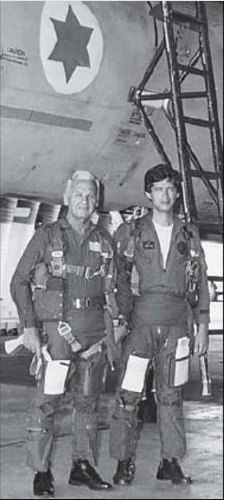
\includegraphics[scale=0.5]{Bekaa_3/WJuR2_4J77s.jpg}
	%	\label{fig:scipion} % Unique label used for referencing the figure in-text\end{document}
	%	%\addcontentsline{toc}{figure}{Figure \ref{fig:placeholder}} % Uncomment to add the figure to the table of contents%----------------------------------------------------------------------------------------
	\caption{Дани и Ронэн}%	CHAPTER 2
\end{figure}

Так вот, 10-го июня же один из F-15 (пилот - Мики Лев, через год будет сбит над Ливаном прямым попаданием зенитного снаряда) крайне неудачно пролетел через облако обломков сбитого им МиГ-21 и получил некоторые повреждения - впрочем, тоже не смертельные, но поволноваться пришлось.

11-го июня сирийцы повторили попытку прорваться к израильским ударникам - и снова неудачно. Большинство было сбито F-15 и F-16. В одном из случаев их перехватил экипаж “Фантома”, патрулировавашего в составе смешанного звена с F-15. В итоге, подполковник Пери Бен-Ами стал последним асом “Фантома” в истории (к тому моменту у него были 4 победы в 73-м - 3 вертолета Ми-8 в первый день войны и МиГ-21). Он был уникальным снайпером даже по понятиям ХельХа Авир — его описывали как летчика, который может стрелять из встроенной пушки «Вулкан" очередями по 8 снарядов, и все шесть положить в летящий над самой землёй вертолёт. Вообще, с ним была связана другая уникальная история. Дело в том, что за несколько лет до описываемых событий у него диагностировали рак. Фактически, Бен-Ами летал со второй стадией. Именно эта болезнь и стала причиной его смерти в 88-м году.

\begin{figure}[h!tb] 
	\centering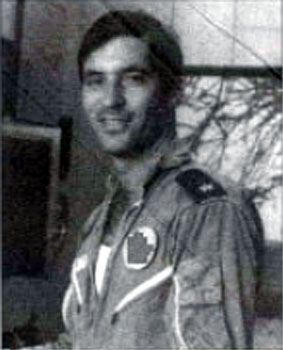
\includegraphics[scale=0.5]{Bekaa_3/ETfLbaXXVqw.jpg}
	%	\label{fig:scipion} % Unique label used for referencing the figure in-text\end{document}
	%	%\addcontentsline{toc}{figure}{Figure \ref{fig:placeholder}} % Uncomment to add the figure to the table of contents%----------------------------------------------------------------------------------------
	\caption{Бен-Ами Пери}%	CHAPTER 2
\end{figure}

Начиная с 9-го июня количество вылетов сирийцев пошло на спад - не совсем понятно, то ли они не хотели рисковать самолетами, то ли не могли поднять в воздух больше. Моральное состояние сирийских летчиков было близким к катастрофе - да это и не удивительно. Когда вы видите, как взлетает эскадрилья - возвращается звено, взлетает восьмерка - возвращается пара, вы всерьез задумаетесь о своих шанса дожить до конца дня. До конца войны израильтяне потерь не понесли. Однако последующие дни они были - 13-го июня, через два дня после начала войны, 2 ракетами С-75 был сбит “Кфир” С.2 из состава воздушной разведки. Эта потеря не имеет отношения к Ливану - целью израильтян был Тартус. В итоге пилот катапультировался при заходе на посадку. 24 июля в долине Бекаа комплексом “Ока” (или “Квадратом”) был сбит RF-4(E) Гиля Фогеля и Аарона Каца. Основной причиной считается расслабленность пилота - он посчитал, что сирийцы уже разбиты и не представляют никакой опасности, за что и поплатился. В итоге он вернулся домой в 74-м, а оператор, опытнейший Аарон Кац, погиб при катапультировании.

11-го июня война (по крайней мере, ее первая стадия) закончилась. Конфликт вспыхнул еще несколько раз с новой силой, в основном - по причине острого желания израильтян добраться таки до трассы Бейрут-Дамаск. Впереди было много всего - Сабра и Шатила, эвакуация ООП, взрывы казарм миротоворцев ... но пока - война закончилась.

Единственной потерей боевых реактивных самолетов стал "Скайхок" Аарона Ахиаза, сбитый палестинцами в первый день войны. Некоторое количество самолетов получило повреждения - в основном от осколков зенитных снарядов и ПЗРК. Сирийцы утверждают, что ими сбито от 20 до 70 израильских самолетов - правда, они не показали ни пленных, ни тел, ни частей сбитых самолетов. Все известные изображения, которые выдают за них - либо датируются 73-м годом, либо к Ливану отношения не имеют, либо сделаны в графическом редакторе.

Потери сирийцев неизвестны - израильтяне претендуют на 80-85 сбитых за войну. Скорее всего, эта цифра несколько завышена, но вряд-ли существенно. Все-таки средства объективного контроля относительно 73-го года ушли далеко вперед.

13 июня случилось невероятное - сирийцам наконец удалось сбить один израильский самолет. Причем даже не над Ливаном - "Кфир" из эскорта фоторазведки был сбит над Латакией. "Квадратом" сбили? Щас - отличился расчет "С-75". Поврежденный самолет пытались сначала посадить с Хайфе, потом в Рамат-Давиде, в итоге при заходе на посадку он стал неуправляемым и пилот катапультировался практически над полосой.

24-го июля сирийцы сбили "Квадратом" "Фантом" фоторазведки - его пилот расслабился и обнаглел вкрай, нарушив полетное задание и в итоге нарвался на засаду - штурман погиб, а пилот попал в плен и в итоге был обменян на пару сотен боевиков.

В ноябре 83-го комэск эскадрильи Кфиров Мики Лев был сбит над Бейрутом - в тот же день его вернули израильтянам. Этот "Кфир" стал последним израильским самолетом, потерянным после воздействия противника.

Война окончилась. От ее результатов офигели все.

В рунете есть два совершенно странных противоположных мнения о результатах Ливанской войны. Согласно одному из них, Израиль одержал величайшую победу, уничтожив сотни советских советников и опозорив советскую армию лично - к сожалению, при чем здесь вообще советская армия, не уточняется. Некоторые авторы идут дальше и ухитряются связать разгром сирийцев в 82-м году и перестройку в СССР - якобы израильская победа показала бесперспективность советского политического строя. Какая здесь связь - сложно представить, спросите у фанатов РЕН-ТВ и “военной тайны”, они специалисты по таким вещам.

Другие утверждения не особо лучше - отдельные товарищи (в основном “советской закалки”) из года в год цитируют газету “Правда”, утверждая, что коварные ЕРЖ скрывают потери десятков самолетов, а от полного разгрома на земле их спасло только вмешательство американской дипломатии - сирийские танки под руководством мудрых советников были готовы загнать сионистскую гадину практически за Можай, в смысле за Негев.

Разумеется, и те и другие крайности выглядят достаточно забавно. Военная победа Израиля была совершенно закономерна - точно так же, как закономерно его итоговое политическое поражение. Для того, чтобы действительно победить, израильтянам нужно было получить в Ливане не полоску земли, а полноценное дружественное правительство - что в условиях Ближнего Востока нереально. Можно было поддерживать Хаддада, Жмайелей и маронитов, да кого угодно - но никто в арабском мире в здравом уме не пошел бы на открытый союз с евреями - особенно в стране, большинство населения которой составляют мусульмане.

В конце концов, даже нишу сбежавших в Тунис арафатовцев очень быстро заняла другая террористическая организация - шиитская “Хезболла”, причем в отличие от ООП, эти ребята организовывали теракты вообще против всех - например, похитили нескольких и убили одного сотрудника советского посольства. Про знаменитые взрывы казарм морпехов можно и не вспоминать.

Ливан был большой пороховой бочкой - и рано или поздно случилась бы Сабра и Шатила - или что-то подобное. К чести израильского общества, трагедия в палестинском анклаве вызвала шквал обвинений в адрес армии и требования разобраться в причинах - на акцию протеста, требующую разобраться в возможной причастности армии к убийству боевиками-маронитами (!) палестинцев (!!) вышло 10% взрослого населения Израиля (!!!). По-сути, в тот момент в глазах общества война была проиграна. В прессе все чаще звучали рассуждения о "колониальной" природе Ливанской войны и пожелания отправить Арика и Бегина в отставку, и кризис внешний сменился кризисом внутренним.

Могли ли сирийцы остановить израильтян? Да - если бы в сирийских танках сидели советские солдаты. Противостоять же израильтянам в воздухе на той технике, которую поставил арабам СССР, было нереально даже для светловолосых друзей с Севера.

Как восприняли события 6-го июня 82-го года в разных странах?

Для Израиля результат превзошел вообще все ожидания. До начала войны ожидались потери - ВВС предполагали “разменять” 1 самолет на 1 батарею ЗРК. Летчики об этом знали - и не сказать, что это знание доставляло им радость. Ко всеобщему удивлению, операция закончилась вообще без потерь. Это был реванш за 73-й год. Для ВВС - своего рода очищение от позора паники первых дней той войны и доказательство того, что они снова могут все - эдакий несокрушимый “меч Давида”.

Сирийцы так и не поняли, что произошло. Они заявили, что сбили десятки “сионистских агрессоров” - я, честно, не знаю, верили они в это утверждение или просто не могли признать очевидного. В первое верится больше.

Но в локальные разборки израильтян и сирийцев были вовлечены два куда более интересных участника - сверхдержавы и лидеры своих военных блоков. СССР и США.

В Союзе как всегда заявили, что советское оружие показало себя достойно. Проблема была в том, что в СССР, в отличие от сирийцев, ОЧЕНЬ хорошо поняли, что произошло, и чем это грозит в будущем. А потому едва ли не сразу в Сирию направились многочисленные комиссии - разбирать, собирать, анализировать. А главное - понять, могут ли подобную операцию провести американцы - уже в Европе против советов. И - разработать меры противодействия. Разбирали очень подробно - вскоре большое внимание операции уделяли даже в училищах транспортной и военно-транспортной авиации.

В советской “открытой” печати было несколько интересных статей. В первую очередь - в 83-м году, в сентябрьском и октябрьском номерах “авиации и космонавтики” вышла статья подполковника Дуброва, “Авиация в ливанском конфликте”. Несмотря на наличие ритуальных штампов в духе “разбойничьего нападения израильской военщины” и “сионистских захватчиков”, она представляет собой на удивление хороший и внятный для своего времени “разбор полетов” - даже если закрыть глаза на ряд досадных ошибок (ну не мог человек в 83-м году знать все то, что знаем мы нынешние) - можно сделать вывод, что в СССР в общем уделяли очень большое внимание той операции.

Для СССР было несколько открытий - в первую очередь, сам тот факт, что операция была проведена под управлением “в реальном времени”. Нам еще предстояло научиться так работать. Кстати, американцам - тоже.

Во-вторых, использование “Хокая” - его разбирала отдельная комиссия. Я не уверен, поняли ли в СССР сразу тот факт, что самолет работал даже не столько командным пунктом, а скорее “глазами” истребительной авиации - принятие решений зачастую выносилось на находящихся в воздухе командиров эскадрилий или отдельных летчиков. Для советской авиации с ее традиционной привязкой к командам с земли нежелательностью проявления инициативы это было чем-то совсем новым.

В-третьих, пересмотр роли истребительной авиации. В Союзе отмечали уход от управления истребителями с земли и непосредственного сопровождения ударной авиации в пользу мобильного заслона и большей тактической свободы.

В общем, в СССР посмотрели, сделали выводы в меру своего понимания происходящего и способности к изменениям.

А что же американцы?

Во-первых, американцы, мягко говоря, удивились. Особенно после того, как в 83-м в одном (!) налете потеряли больше самолетов, чем Израиль за всю Ливанскую войну.

Во-вторых, в ВВС выпустили огромное количество материалов в попытке осмыслить произошедшее и с максимальной пользой “переложить” идеи израильтян на свои ВВС. Наиболее точно настроения американцев можно передать фразой из одного такого отчета - “мы много лет помогали Израилю - пора, наконец, что-то получить от них”. Этим “что-то” оказался бесценный опыт и переосмысление операций по подавлению ЗРК.

Остановимся более подробно на двух американских работах.
Первая была написана майором Дэвидом Клэри из командно-штабного колледжа ВВС и называлась просто - “Bekaa Valley - Case study. Insights into tomorrow” (полный список ссылок будет в конце поста). Майор Клэри, в общем, приводит к одной очень здравой мысли - успех операции был обусловлен совокупностью факторов - технических, политических, географических - и делать какие-то грандиозные выводы из такой небольшой войны как Ливанская - опасно и безответственно. Операция в Бекаа была весьма ограниченной - как по времени, так и по географии, проходила в уникальных условиях и рассматривать её нужно в первую очередь как победу израильской “системы” над сирийской “системой”. Любая попытка спроецировать её результат на советско-американское противостояние может привести к массе ошибочных выводов.

Вторая - “Уроки Москвы из Ливанской войны 82 года”, Бенджамина Ламбета из корпорации RAND (военные консультанты), разбирает вышеупомянутую советскую статью “Авиации и космонавтики” - в весьма критичной манере, но тоже очень любопытно. Я не буду пересказывать ее содержание - проще прочитать.

А какие выводы можем сделать мы?

Во-первых, не стоит делать глобальных выводов о слабости советского ПВО по одному, пусть и крупному поражению. Тем более - поражению не советских, а сирийских военных. Все современники прекрасно понимали различия между русскими и арабами - и не рисковали недооценивать русских по поражению их бестолковых протеже.

Во-вторых, не стоит делать глобальных выводов о силе и возможностях стран НАТО. Прозвучит странно, но в начале 80-х между американцами и израильтянами во-многих аспектах войны в воздухе была пропасть - не в пользу первых.

В-третьих, скорее всего, сирийцев не спасло бы даже все ПВО Московского округа - скорее всего, в Бекаа израильтяне точно так же раздавили бы его - пусть и не без потерь и “в другие деньги”. Почему? Потому что география. Вряд ли на европейском ТВД популярным способом поражения ПВО могли стать корректируемые артиллерийские снаряды. Да и Ливанского хребта, за которым израильтяне прятались от радаров, снижая время на реакцию сирийских “Квадратов” до считанных минут, там нет.

В-четвертых. Американцы в 83-м попытались повторить отдельные подвиги израильских ВВС. Результат? Провал. За один налет потеряно 2 машины сбитыми и несколько было повреждено. Как так получилось? А вот так. В Мирамаре учат далеко не всему тому, чему учат в Хацерим, как выяснилось. Американцы бросились разбираться - как так! Евреи смогли, а мы нет?! Научились ли янки? Не знаю, спросите у Саддама и Слободана.

А самый главный вывод - да, современная техника - это прекрасно. Но - воюет не она. Воюют люди. Воюют школы- обучения летчиков, обучения механиков, инженерные. К началу 80-х Израиль уже имел неплохую собственную авиаиндустрию (пусть и с большой поддержкой американцев и французов), производя многие компоненты для своих самолетов самостоятельно. И даже - пытаясь производить собственные самолеты (вспоминаем “Лави”). Более того, в 80-х уже американцы многому учились в Израиле и воспринимали их как равных партнеров.

Мог ли СССР назвать Сирию равноправным партнером? Могли ли советские инженеры чему-то научиться у сирийцев? Летчики? Риторический вопрос, правда?

Отсюда - мораль всей этой истории. Побеждает не оружие. Побеждают люди. 

\rule{10cm}{1pt}
Прошел год.
Небо над мирной арабской хатой отдали в руки шурави - так всем стало спокойнее. В первый раз, что ли?..
Евреи вляпались в Сабру и Шатилу и внутриполитический кризис. Им стало не до Ливана.
Вместо ООП в Ливане завились шиитские радикалы из "Хезболлы" и паразиты помельче.
Американцы начали разрабатывать новую концепцию применения авиации.
СССР потерял несколько контрактов на поставку самолетов за рубеж.
США приобрели несколько контрактов на поставку самолетов за рубеж.
...
Арабы так ничему и не научились.

Для дальнейшего чтения:
\begin{enumerate}
	\item  Исследование командно-штабного колледжа ВВС США (англ.) \url{http://www.dtic.mil/dtic/tr/fulltext/u2/a192545.pdf}
Moscow’s lessons for Bekaa - (англ.) \url{https://www.rand.org/content/dam/rand/pubs/reports/2007/R3000.pdf}
\item Архив журнала “Авиация и Космонавтика” за 1983 год \url{https://www.booksite.ru/avia/1983/1983_10.pdf}
\item Хорошее общее описание события (англ.) http://www.airbase.ru/alpha/b/bekaa1/eng/
\item Интервью автору одного из израильских пилотов с подробным разбором событий (там же есть 2 часть) \url{https://fakel-history.ru/intervyu-pilota-izrailskix-vvs-1/}
\item Графомания автора на тему модернизации ВВС Израиля конца 70-х
\url{https://fakel-history.ru/mech_davida_chast1/}
\item Подробный разбор действий эскадрильи “Скайхоков” \url{http://forums.airbase.ru/2006/03/t37615--dolina-bekaa-1982.html}
\item Тема на “Варонлайне”
\item Старый разбор на форуме Авиабазы \url{http://forums.airbase.ru/2006/03/t37615--dolina-bekaa-1982.html}
\item Арабское видение произошедшего (ар.) \url{https://defense-arab.com/vb/threads/116224/page-3?__cf_chl_jschl_tk__=pmd_0f5F41I5Psf5k8IucNnlupEEIIpmV4RNGgJrP6uYmi8-1629529221-0-gqNtZGzNAiWjcnBszQd9}
\item Статья на ВКО про роль РТВ и РТР 
\item Интервью Давида Иври (ивр.) 
\item Разбор полетов от советника эскадрильи МиГ-23 Владимира Бабича (писалось со слов сирийцев, фильтровать победные реляции надобно) \url{http://airwar.ru/history/locwar/bv/mig23mf/mig23mf.html}
\item Shlomo Aloni, «Israeli Phantom II aces» (англ.)

\item сайты «Махиа Шхаким» (ивр.) (\url{sky-high.co.il}, Авиноам Мисников и Амир Сегев), \url{merchav-aviri.org} (ивр.) и \url{group73historians.com} (араб.)
\end{enumerate}

Ссылка на оригинал \url{https://vk.com/wall-162479647_24527}

К оглавлению на странице \pageref{tablecont}